% Options for packages loaded elsewhere
\PassOptionsToPackage{unicode}{hyperref}
\PassOptionsToPackage{hyphens}{url}
\PassOptionsToPackage{dvipsnames,svgnames,x11names}{xcolor}
%
\documentclass[
  letterpaper,
  DIV=11,
  numbers=noendperiod]{scrartcl}

\usepackage{amsmath,amssymb}
\usepackage{iftex}
\ifPDFTeX
  \usepackage[T1]{fontenc}
  \usepackage[utf8]{inputenc}
  \usepackage{textcomp} % provide euro and other symbols
\else % if luatex or xetex
  \usepackage{unicode-math}
  \defaultfontfeatures{Scale=MatchLowercase}
  \defaultfontfeatures[\rmfamily]{Ligatures=TeX,Scale=1}
\fi
\usepackage{lmodern}
\ifPDFTeX\else  
    % xetex/luatex font selection
\fi
% Use upquote if available, for straight quotes in verbatim environments
\IfFileExists{upquote.sty}{\usepackage{upquote}}{}
\IfFileExists{microtype.sty}{% use microtype if available
  \usepackage[]{microtype}
  \UseMicrotypeSet[protrusion]{basicmath} % disable protrusion for tt fonts
}{}
\makeatletter
\@ifundefined{KOMAClassName}{% if non-KOMA class
  \IfFileExists{parskip.sty}{%
    \usepackage{parskip}
  }{% else
    \setlength{\parindent}{0pt}
    \setlength{\parskip}{6pt plus 2pt minus 1pt}}
}{% if KOMA class
  \KOMAoptions{parskip=half}}
\makeatother
\usepackage{xcolor}
\setlength{\emergencystretch}{3em} % prevent overfull lines
\setcounter{secnumdepth}{-\maxdimen} % remove section numbering
% Make \paragraph and \subparagraph free-standing
\ifx\paragraph\undefined\else
  \let\oldparagraph\paragraph
  \renewcommand{\paragraph}[1]{\oldparagraph{#1}\mbox{}}
\fi
\ifx\subparagraph\undefined\else
  \let\oldsubparagraph\subparagraph
  \renewcommand{\subparagraph}[1]{\oldsubparagraph{#1}\mbox{}}
\fi

\usepackage{color}
\usepackage{fancyvrb}
\newcommand{\VerbBar}{|}
\newcommand{\VERB}{\Verb[commandchars=\\\{\}]}
\DefineVerbatimEnvironment{Highlighting}{Verbatim}{commandchars=\\\{\}}
% Add ',fontsize=\small' for more characters per line
\usepackage{framed}
\definecolor{shadecolor}{RGB}{241,243,245}
\newenvironment{Shaded}{\begin{snugshade}}{\end{snugshade}}
\newcommand{\AlertTok}[1]{\textcolor[rgb]{0.68,0.00,0.00}{#1}}
\newcommand{\AnnotationTok}[1]{\textcolor[rgb]{0.37,0.37,0.37}{#1}}
\newcommand{\AttributeTok}[1]{\textcolor[rgb]{0.40,0.45,0.13}{#1}}
\newcommand{\BaseNTok}[1]{\textcolor[rgb]{0.68,0.00,0.00}{#1}}
\newcommand{\BuiltInTok}[1]{\textcolor[rgb]{0.00,0.23,0.31}{#1}}
\newcommand{\CharTok}[1]{\textcolor[rgb]{0.13,0.47,0.30}{#1}}
\newcommand{\CommentTok}[1]{\textcolor[rgb]{0.37,0.37,0.37}{#1}}
\newcommand{\CommentVarTok}[1]{\textcolor[rgb]{0.37,0.37,0.37}{\textit{#1}}}
\newcommand{\ConstantTok}[1]{\textcolor[rgb]{0.56,0.35,0.01}{#1}}
\newcommand{\ControlFlowTok}[1]{\textcolor[rgb]{0.00,0.23,0.31}{#1}}
\newcommand{\DataTypeTok}[1]{\textcolor[rgb]{0.68,0.00,0.00}{#1}}
\newcommand{\DecValTok}[1]{\textcolor[rgb]{0.68,0.00,0.00}{#1}}
\newcommand{\DocumentationTok}[1]{\textcolor[rgb]{0.37,0.37,0.37}{\textit{#1}}}
\newcommand{\ErrorTok}[1]{\textcolor[rgb]{0.68,0.00,0.00}{#1}}
\newcommand{\ExtensionTok}[1]{\textcolor[rgb]{0.00,0.23,0.31}{#1}}
\newcommand{\FloatTok}[1]{\textcolor[rgb]{0.68,0.00,0.00}{#1}}
\newcommand{\FunctionTok}[1]{\textcolor[rgb]{0.28,0.35,0.67}{#1}}
\newcommand{\ImportTok}[1]{\textcolor[rgb]{0.00,0.46,0.62}{#1}}
\newcommand{\InformationTok}[1]{\textcolor[rgb]{0.37,0.37,0.37}{#1}}
\newcommand{\KeywordTok}[1]{\textcolor[rgb]{0.00,0.23,0.31}{#1}}
\newcommand{\NormalTok}[1]{\textcolor[rgb]{0.00,0.23,0.31}{#1}}
\newcommand{\OperatorTok}[1]{\textcolor[rgb]{0.37,0.37,0.37}{#1}}
\newcommand{\OtherTok}[1]{\textcolor[rgb]{0.00,0.23,0.31}{#1}}
\newcommand{\PreprocessorTok}[1]{\textcolor[rgb]{0.68,0.00,0.00}{#1}}
\newcommand{\RegionMarkerTok}[1]{\textcolor[rgb]{0.00,0.23,0.31}{#1}}
\newcommand{\SpecialCharTok}[1]{\textcolor[rgb]{0.37,0.37,0.37}{#1}}
\newcommand{\SpecialStringTok}[1]{\textcolor[rgb]{0.13,0.47,0.30}{#1}}
\newcommand{\StringTok}[1]{\textcolor[rgb]{0.13,0.47,0.30}{#1}}
\newcommand{\VariableTok}[1]{\textcolor[rgb]{0.07,0.07,0.07}{#1}}
\newcommand{\VerbatimStringTok}[1]{\textcolor[rgb]{0.13,0.47,0.30}{#1}}
\newcommand{\WarningTok}[1]{\textcolor[rgb]{0.37,0.37,0.37}{\textit{#1}}}

\providecommand{\tightlist}{%
  \setlength{\itemsep}{0pt}\setlength{\parskip}{0pt}}\usepackage{longtable,booktabs,array}
\usepackage{calc} % for calculating minipage widths
% Correct order of tables after \paragraph or \subparagraph
\usepackage{etoolbox}
\makeatletter
\patchcmd\longtable{\par}{\if@noskipsec\mbox{}\fi\par}{}{}
\makeatother
% Allow footnotes in longtable head/foot
\IfFileExists{footnotehyper.sty}{\usepackage{footnotehyper}}{\usepackage{footnote}}
\makesavenoteenv{longtable}
\usepackage{graphicx}
\makeatletter
\def\maxwidth{\ifdim\Gin@nat@width>\linewidth\linewidth\else\Gin@nat@width\fi}
\def\maxheight{\ifdim\Gin@nat@height>\textheight\textheight\else\Gin@nat@height\fi}
\makeatother
% Scale images if necessary, so that they will not overflow the page
% margins by default, and it is still possible to overwrite the defaults
% using explicit options in \includegraphics[width, height, ...]{}
\setkeys{Gin}{width=\maxwidth,height=\maxheight,keepaspectratio}
% Set default figure placement to htbp
\makeatletter
\def\fps@figure{htbp}
\makeatother

\KOMAoption{captions}{tableheading}
\makeatletter
\makeatother
\makeatletter
\makeatother
\makeatletter
\@ifpackageloaded{caption}{}{\usepackage{caption}}
\AtBeginDocument{%
\ifdefined\contentsname
  \renewcommand*\contentsname{Table of contents}
\else
  \newcommand\contentsname{Table of contents}
\fi
\ifdefined\listfigurename
  \renewcommand*\listfigurename{List of Figures}
\else
  \newcommand\listfigurename{List of Figures}
\fi
\ifdefined\listtablename
  \renewcommand*\listtablename{List of Tables}
\else
  \newcommand\listtablename{List of Tables}
\fi
\ifdefined\figurename
  \renewcommand*\figurename{Figure}
\else
  \newcommand\figurename{Figure}
\fi
\ifdefined\tablename
  \renewcommand*\tablename{Table}
\else
  \newcommand\tablename{Table}
\fi
}
\@ifpackageloaded{float}{}{\usepackage{float}}
\floatstyle{ruled}
\@ifundefined{c@chapter}{\newfloat{codelisting}{h}{lop}}{\newfloat{codelisting}{h}{lop}[chapter]}
\floatname{codelisting}{Listing}
\newcommand*\listoflistings{\listof{codelisting}{List of Listings}}
\makeatother
\makeatletter
\@ifpackageloaded{caption}{}{\usepackage{caption}}
\@ifpackageloaded{subcaption}{}{\usepackage{subcaption}}
\makeatother
\makeatletter
\@ifpackageloaded{tcolorbox}{}{\usepackage[skins,breakable]{tcolorbox}}
\makeatother
\makeatletter
\@ifundefined{shadecolor}{\definecolor{shadecolor}{rgb}{.97, .97, .97}}
\makeatother
\makeatletter
\makeatother
\makeatletter
\makeatother
\ifLuaTeX
  \usepackage{selnolig}  % disable illegal ligatures
\fi
\IfFileExists{bookmark.sty}{\usepackage{bookmark}}{\usepackage{hyperref}}
\IfFileExists{xurl.sty}{\usepackage{xurl}}{} % add URL line breaks if available
\urlstyle{same} % disable monospaced font for URLs
\hypersetup{
  pdftitle={TP2- Étude de l'évolution du niveau de partisanerie des jeunes entre la cohorte de 1988 et de 2021 (Option 2)},
  pdfauthor={Olivia Saffioti},
  colorlinks=true,
  linkcolor={blue},
  filecolor={Maroon},
  citecolor={Blue},
  urlcolor={Blue},
  pdfcreator={LaTeX via pandoc}}

\title{TP2- Étude de l'évolution du niveau de partisanerie des jeunes
entre la cohorte de 1988 et de 2021 (Option 2)}
\author{Olivia Saffioti}
\date{2024-05-02}

\begin{document}
\maketitle
\ifdefined\Shaded\renewenvironment{Shaded}{\begin{tcolorbox}[frame hidden, borderline west={3pt}{0pt}{shadecolor}, boxrule=0pt, interior hidden, breakable, sharp corners, enhanced]}{\end{tcolorbox}}\fi

\hypertarget{introduction}{%
\subsection{Introduction}\label{introduction}}

« La tendance à la baisse (du taux de participation des Québécois)
observée depuis plusieurs années s'explique en grande partie par le fait
que les électeurs des plus récentes cohortes votent moins que ceux des
cohortes antérieures. Les jeunes seraient donc en partie responsables du
déclin de la participation électorale au Québec » a expliqué
l'organisation Élections Québec dans un article de presse de LEDEVOIR en
2018 (Rettino-Parazelli 2018). Ces propos mettent l'emphase sur un
phénomène typique des démocraties contemporaines : les jeunes
constituent le groupe social qui vote le moins (Rettino-Parazelli 2018).
Or, la littérature scientifique établit un lien entre le vote et la
partisanerie. En effet, de nos jours, les personnes âgées sont
généralement plus loyales envers un parti politique que les jeunes.
Selon la théorie de la mobilisation cognitive, les plus jeunes sont
aujourd'hui plus critiques vis -à -vis des partis politiques en raison
de la transformation des médias de masse, ou encore d'un accès plus
facile à la connaissance (Lisi 2015, 496). Ils sont donc plus volatiles
et ont une identité partisane plus faible (Lisi 2015, 495). Cependant,
des recherches américaines ont montré que le niveau de partisanerie des
jeunes ne dépendait pas forcément de l'âge mais plutôt de leur
génération d'appartenance (ou cohortes) (Converse 1976; Abramson 1976).
En effet, le niveau de partisanerie des jeunes américains déclinerait de
plus en plus au fil des générations (Abramson 1976). De plus, les études
comparatives existantes ont donné peu d'attention aux dynamiques des
identités partisanes au fil du temps (Lisi 2015, 494). Or, les
dynamiques temporelles sont importantes pour comprendre l'évolution de
l'attachement partisan, surtout au vu de la mutation des sociétés
contemporaines (Lisi 2015, 494). Il semble donc pertinent de mener une
étude transversale comparative sur le niveau de partisanerie entre deux
cohortes de jeunes. Cette méthode vise à ``connaître les situations, les
pratiques, et les opinions des personnes interrogées à un moment
donné''(Paugam 2010). Il apparaît également intéressant de se centrer
sur un autre pays que les États-Unis. C'est pourquoi, nous avons décidé
de nous centrer sur le cas du Canada, dont le contexte politique et
culturel montre une importance de la partisanerie au sein des provinces
comme le Québec (Veilleux 2022) . Ainsi, nous étudierons comment
l'identité partisane des jeunes canadiens a évolué d'une cohorte à une
autre. Pour ce faire, nous mobiliserons deux sondages : celui des
élections canadiennes de 1988 et celui des élections canadiennes de
2021. Nous avons choisi ces deux bases de données car elles mobilisent
les mêmes variables (âge, niveau d'identification partisane, etc.) et
sont faciles d'accès. En outre, elles nous permettront d'étudier le
niveau de partisanerie de deux cohortes de jeunes, séparées à plusieurs
dizaines d'années d'intervale. Nous comparerons les données de ces
sondages afin d'analyser comment le niveau de partisanerie des jeunes a
évolué. Pour cela, nous croiserons ces deux bases de données et
élaborerons un graphique afin de visualiser les données.

\hypertarget{hypothuxe8se}{%
\subsection{Hypothèse}\label{hypothuxe8se}}

L'hypothèse défendue par notre étude est celle que les jeunes de 1988
étaient plus partisans que les jeunes de 2021.

\hypertarget{donnuxe9es-et-muxe9thodes}{%
\subsection{Données et méthodes}\label{donnuxe9es-et-muxe9thodes}}

Tout d'abord, nous avons nettoyé nos bases de données. Nous avons
commencé par créer de nouvelles bases de données avec seulement les
variables que nous voulions conserver. Il s'agit des bases de données
Elections\_2021\_nouveau et Elections\_1988\_new. Nous avons décidé de
conserver les variables de l'age des répondants, leur niveau
d'identification à un parti politique, le parti politique auquel ils
s'affilient, et l'année de naissance. L'année de naissance a été
conservée uniquement au sein de la base de données Elections\_1988\_new
afin de calculer l'âge des répondants en fonction de cette variable. En
effet, la base de données de 2021 avait déjà une variable indiquant
l'age des répondants, ce qui n'était pas le cas de la banque de données
de 1988. Ainsi, nous avons soustrait l'année de naissance à 1988
(l'année du sondage) via la fonction '' mutate'' afin d'obtenir les âges
de tous les répondants. Nous avons ensuite renommé les variables
``Niveau\_identification'', ``age\_du\_répondant'',
``intérêt\_élections\_fédérales'', et ``Identité\_partisane'' grâce à la
fonction ``rename''. Par la suite, pour la base de données de 2021, nous
avons supprimé toutes les valeurs de la variable Niveau\_identification
qui étaient égales à NA (soit dont la donnée était inexistente). Pour
cela nous avons mobilisé la fonction ``filter''. Nous avons fait de même
avec la base de données de 1988 pour les variables age\_du\_répondant et
Niveau\_identification. Nous avons également conservé uniquement les
âges entre 18 et 30 ans dans les deux bases de données (soit les
répondants considérés comme ``jeunes''). Dans la base de données de
1988, nous avons recodé la variable Niveau\_identification afin
d'harmoniser son échelle de mesure avec celle de la base de données de
2021. Pour cela, nous avons utilisé la fonction ``mutate'' et
``recode''. Puis, nous avons recoder à nouveau cette variable dans les
deux bases de données afin que le graphique que nous allions produire
plus tard apparaisse plus clair et compréhensible. Ainsi, l'échelle de
mesure de la variable Niveau\_identification est devenue dans les deux
bases de données : 1 = Ne sais pas/refus, 2 = pas très fort, 3= assez
fort, 4= très fort; alors qu'auparavant le code était inversé comme suit
: 4 = ne sais pas/refus, 3 = pas très fort, 2 = assez fort, 1 = très
fort. Par la suite, nous avons créé une nouvelle colonne dans les bases
de données de 2021 et de 1988 qui mettait en exergue le pourcentage de
fois où les jeunes de 18 à 30 ans se sont identifiés aux niveaux de
partisanerie. Il s'agissait de savoir combien de jeunes, en pourcentage,
ont répondu 1, 2, 3, ou 4 (les valeurs de l'échelle de mesure). Cela
nous permettait de rendre compte des proportions de jeunes qui ont un
niveau de partisanerie très fort, assez fort, pas très fort, et de la
proportion de jeunes qui ne savaient pas ou qui ont refusé de répondre.
Pour cela nous avons mobilisé les fonctions ``group\_by'', ``summarise''
et ``nrow''. En outre, nous avions besoin de ces pourcentages afin de
générer un graphique clair, représentant la relation entre les cohortes
de jeunes et le niveau de partisanerie. Enfin, nous avons créé une autre
colonne dans chaque base de données afin de spécifier l'année du sondage
à laquelle les données sont référées. Cela nous permettait par la suite
de fusionner nos bases de données, tout en repérant quelles données sont
issues de 1988 et de 2021. Finalement, nous avons croisé nos deux bases
de données à partir des variables ``Pourcentage'',
``Niveau\_identification'', et ``année du sondage''. Pour cela nous
avons utilisé la fonction ``merge''. Nous avons élaboré notre graphique
à partir de cette nouvelle base de données.

\hypertarget{ruxe9sultats}{%
\subsection{Résultats}\label{ruxe9sultats}}

Nous avons élaboré le graphique ci-dessous à partir de la base de
données croisant les sondages de 1988 et de 2021. Elle se nomme
``Données\_pourcentage\_Elections\_croisées''. À l'intérieur de cette
base de données, 2902 observations étaient représentées sous forme de 7
pourcentages.

\begin{figure}

{\centering \includegraphics{/Users/oliviasaffioti/Desktop/Graph2bis.png}

}

\caption{Graphique comparant les niveaux de partisanerie des cohortes de
jeunes}

\end{figure}

Les résultats exposés dans le graphique indiquent qu'il semblerait y
avoir une tendance pour des niveaux de partisanrie plus élevés en 2021
par rapport à 1988. En effet, en 2021, 2,4\% des jeunes ne savaient pas
ou ont refusé de communiquer leur niveau de partisanerie.
Comparativement, aucun jeune de 18 à 30 ans n'a pas répondu ou a refusé
de communiquer son degré de partisanerie. En outre, 16\% des jeunes en
2021 s'identifiaient à un niveau de partisanerie ``pas très fort'',
contre 21,7\% des jeunes en 1988. Il y avait donc plus de jeunes en 1988
qui avaient un niveau de partisanerie ``pas très fort''. De surcroît,
53,8 \% des jeunes de 2021 s'identifiaient à un niveau de partisanerie
``assez fort'', contre 58,6\% en 1988. Il y avait donc davantage de
jeunes avec une identité partisane ``assez forte'' en 1988 par rapport à
2021. En revanche, 27,8\% des jeunes en 2021 s'identifiaient à un niveau
de partisanerie ``très fort'', contre 19,6\% des jeunes en 1988.
Autrement dit, il y avait plus de jeunes dont l'identité partisane était
``très forte'' en 2021 comparé à 1988.

Ainsi, il semblerait que notre hypothèse soit inférée. Les résultats
obtenus sont contraires à ceux des études antérieures menées aux
États-Unis. Cependant, ces résultats pourraient résulter du fait que les
échantillons des bases de données de 1988 et de 2021 ne contiennent pas
le même nombre d'observations. En effet, la base de données de 2021
contient 2566 observations après nettoyage contre 336 observations pour
la base de données de 1988. Si les échantillons avaient été plus
proportionnels, nous aurions pu trouver une autre tendance quant à
l'évolution du niveau de partisanerie des jeunes entre 1988 et 2021.

\hypertarget{annexe}{%
\subsection{Annexe}\label{annexe}}

\begin{Shaded}
\begin{Highlighting}[]
\CommentTok{\# Libraries}

\FunctionTok{library}\NormalTok{(tidyverse)}
\end{Highlighting}
\end{Shaded}

\begin{verbatim}
-- Attaching core tidyverse packages ------------------------ tidyverse 2.0.0 --
v dplyr     1.1.4     v readr     2.1.4
v forcats   1.0.0     v stringr   1.5.1
v ggplot2   3.4.4     v tibble    3.2.1
v lubridate 1.9.3     v tidyr     1.3.0
v purrr     1.0.2     
-- Conflicts ------------------------------------------ tidyverse_conflicts() --
x dplyr::filter() masks stats::filter()
x dplyr::lag()    masks stats::lag()
i Use the conflicted package (<http://conflicted.r-lib.org/>) to force all conflicts to become errors
\end{verbatim}

\begin{Shaded}
\begin{Highlighting}[]
\CommentTok{\# Définir le répertoire de travail et importer les bases de données sur Rstudio}

\FunctionTok{setwd}\NormalTok{(}\StringTok{"/Users/oliviasaffioti/Desktop/fas\_1001\_Saffioti/\_tp/TP2 (FAS 1001)"}\NormalTok{)}
\FunctionTok{getwd}\NormalTok{()}
\end{Highlighting}
\end{Shaded}

\begin{verbatim}
[1] "/Users/oliviasaffioti/Desktop/fas_1001_Saffioti/_tp/TP2 (FAS 1001)"
\end{verbatim}

\begin{Shaded}
\begin{Highlighting}[]
\NormalTok{Elections\_2021 }\OtherTok{\textless{}{-}} \FunctionTok{read.csv}\NormalTok{(}\StringTok{"Canadian\_Election\_Study\_2021.csv"}\NormalTok{, }\AttributeTok{sep =} \StringTok{","}\NormalTok{)}
\NormalTok{Elections\_1988 }\OtherTok{\textless{}{-}} \FunctionTok{read.csv}\NormalTok{(}\StringTok{"Canadian\_Election\_Study\_1988.csv"}\NormalTok{, }\AttributeTok{sep =}\StringTok{","}\NormalTok{)}

\CommentTok{\#Nettoyer la base de données de 2021}

\NormalTok{Elections\_2021\_nouveau }\OtherTok{\textless{}{-}}\NormalTok{ Elections\_2021[, }\FunctionTok{c}\NormalTok{(}\StringTok{"cps21\_yob"}\NormalTok{, }\StringTok{"cps21\_yob\_2003\_age"}\NormalTok{, }\StringTok{"cps21\_age"}\NormalTok{, }\StringTok{"cps21\_interest\_gen\_1"}\NormalTok{, }\StringTok{"cps21\_interest\_elxn\_1"}\NormalTok{, }\StringTok{"cps21\_fed\_id"}\NormalTok{, }\StringTok{"cps21\_fed\_id\_str"}\NormalTok{)]}
\NormalTok{Elections\_2021\_nouveau }\OtherTok{\textless{}{-}}\NormalTok{ Elections\_2021\_nouveau }\SpecialCharTok{\%\textgreater{}\%} \FunctionTok{rename}\NormalTok{(}\StringTok{"age\_du\_répondant"} \OtherTok{=} \StringTok{"cps21\_age"}\NormalTok{, }\StringTok{"Niveau\_identification"} \OtherTok{=} \StringTok{"cps21\_fed\_id\_str"}\NormalTok{, }\StringTok{"Identité\_partisane"} \OtherTok{=} \StringTok{"cps21\_fed\_id"}\NormalTok{)}
\NormalTok{Elections\_2021\_nouveau }\OtherTok{=}\NormalTok{ Elections\_2021\_nouveau }\SpecialCharTok{|\textgreater{}} \FunctionTok{filter}\NormalTok{(}\SpecialCharTok{!}\FunctionTok{is.na}\NormalTok{(Niveau\_identification))}
\NormalTok{Elections\_2021\_nouveau }\OtherTok{=}\NormalTok{ Elections\_2021\_nouveau }\SpecialCharTok{|\textgreater{}} \FunctionTok{filter}\NormalTok{(age\_du\_répondant }\SpecialCharTok{\textless{}=} \DecValTok{30}\NormalTok{)}
\NormalTok{Elections\_2021\_nouveau }\OtherTok{\textless{}{-}}\NormalTok{ Elections\_2021\_nouveau }\SpecialCharTok{\%\textgreater{}\%} \FunctionTok{mutate}\NormalTok{(}\AttributeTok{Niveau\_identification =} \FunctionTok{recode}\NormalTok{(Niveau\_identification, }\StringTok{"1"} \OtherTok{=} \StringTok{"4"}\NormalTok{, }\StringTok{"2"} \OtherTok{=} \StringTok{"3"}\NormalTok{, }\StringTok{"3"} \OtherTok{=} \StringTok{"2"}\NormalTok{, }\StringTok{"4"} \OtherTok{=} \StringTok{"1"}\NormalTok{))}
\NormalTok{Elections\_2021\_nouveau2}\FloatTok{.0} \OtherTok{\textless{}{-}}\NormalTok{ Elections\_2021\_nouveau }\SpecialCharTok{\%\textgreater{}\%} \FunctionTok{group\_by}\NormalTok{(Niveau\_identification) }\SpecialCharTok{\%\textgreater{}\%} \FunctionTok{summarise}\NormalTok{(}\AttributeTok{Pourcentage =} \FunctionTok{n}\NormalTok{() }\SpecialCharTok{/} \FunctionTok{nrow}\NormalTok{(Elections\_2021\_nouveau) }\SpecialCharTok{*} \DecValTok{100}\NormalTok{)}
\NormalTok{Elections\_2021\_nouveau2}\FloatTok{.0}\NormalTok{[}\StringTok{"année du sondage"}\NormalTok{] }\OtherTok{=} \DecValTok{2021}

\CommentTok{\# Nettoyer la base de données de 1988}

\NormalTok{Elections\_1988\_new }\OtherTok{\textless{}{-}}\NormalTok{ Elections\_1988 [, }\FunctionTok{c}\NormalTok{(}\StringTok{"yrbirth"}\NormalTok{, }\StringTok{"xl4"}\NormalTok{, }\StringTok{"xl5"}\NormalTok{)]}
\NormalTok{Elections\_1988\_new }\OtherTok{\textless{}{-}}\NormalTok{ Elections\_1988\_new }\SpecialCharTok{\%\textgreater{}\%} \FunctionTok{mutate}\NormalTok{(}\AttributeTok{age =} \DecValTok{1988} \SpecialCharTok{{-}}\NormalTok{ yrbirth)}
\NormalTok{Elections\_1988\_new2 }\OtherTok{\textless{}{-}}\NormalTok{ Elections\_1988\_new }\SpecialCharTok{\%\textgreater{}\%} \FunctionTok{mutate}\NormalTok{(}\AttributeTok{Niveau\_identification =} \FunctionTok{recode}\NormalTok{(xl5, }\StringTok{"1"} \OtherTok{=} \StringTok{"1"}\NormalTok{, }\StringTok{"3"} \OtherTok{=} \StringTok{"2"}\NormalTok{, }\StringTok{"5"} \OtherTok{=} \StringTok{"3"}\NormalTok{, }\StringTok{"9"} \OtherTok{=} \StringTok{"4"}\NormalTok{, }\StringTok{"8"} \OtherTok{=} \StringTok{"4"}\NormalTok{ ))}
\NormalTok{Elections\_1988\_new2 }\OtherTok{\textless{}{-}}\NormalTok{ Elections\_1988\_new2 }\SpecialCharTok{\%\textgreater{}\%} \FunctionTok{rename}\NormalTok{(}\StringTok{"année\_de\_naissance"} \OtherTok{=}\StringTok{"yrbirth"}\NormalTok{, }\StringTok{"age\_du\_répondant"} \OtherTok{=} \StringTok{"age"}\NormalTok{, }\StringTok{"Identité\_partisane"} \OtherTok{=} \StringTok{"xl4"}\NormalTok{, }\StringTok{"Codage\_originel\_niveau\_identification"} \OtherTok{=} \StringTok{"xl5"}\NormalTok{)}
\NormalTok{Elections\_1988\_new2 }\OtherTok{=}\NormalTok{ Elections\_1988\_new2 }\SpecialCharTok{|\textgreater{}} \FunctionTok{filter}\NormalTok{(}\SpecialCharTok{!}\FunctionTok{is.na}\NormalTok{(Niveau\_identification))}
\NormalTok{Elections\_1988\_new2 }\OtherTok{=}\NormalTok{ Elections\_1988\_new2 }\SpecialCharTok{|\textgreater{}} \FunctionTok{filter}\NormalTok{(}\SpecialCharTok{!}\FunctionTok{is.na}\NormalTok{(age\_du\_répondant))}
\NormalTok{Elections\_1988\_new2 }\OtherTok{=}\NormalTok{ Elections\_1988\_new2 }\SpecialCharTok{|\textgreater{}} \FunctionTok{filter}\NormalTok{(age\_du\_répondant }\SpecialCharTok{\textless{}=} \DecValTok{30}\NormalTok{)}
\NormalTok{Elections\_1988\_new2 }\OtherTok{\textless{}{-}}\NormalTok{ Elections\_1988\_new2 }\SpecialCharTok{\%\textgreater{}\%} \FunctionTok{mutate}\NormalTok{(}\AttributeTok{Niveau\_identification =} \FunctionTok{recode}\NormalTok{(Niveau\_identification, }\StringTok{"1"} \OtherTok{=} \StringTok{"4"}\NormalTok{, }\StringTok{"2"} \OtherTok{=} \StringTok{"3"}\NormalTok{, }\StringTok{"3"} \OtherTok{=} \StringTok{"2"}\NormalTok{, }\StringTok{"4"} \OtherTok{=} \StringTok{"1"}\NormalTok{))}
\NormalTok{Elections\_1988\_new2 }\OtherTok{=}\NormalTok{ Elections\_1988\_new2 }\SpecialCharTok{|\textgreater{}} \FunctionTok{filter}\NormalTok{(age\_du\_répondant }\SpecialCharTok{!=} \DecValTok{16}\NormalTok{)}
\NormalTok{Elections\_1988\_new2}\FloatTok{.0} \OtherTok{\textless{}{-}}\NormalTok{ Elections\_1988\_new2 }\SpecialCharTok{\%\textgreater{}\%} \FunctionTok{group\_by}\NormalTok{(Niveau\_identification) }\SpecialCharTok{\%\textgreater{}\%} \FunctionTok{summarise}\NormalTok{(}\AttributeTok{Pourcentage =} \FunctionTok{n}\NormalTok{() }\SpecialCharTok{/} \FunctionTok{nrow}\NormalTok{(Elections\_1988\_new2) }\SpecialCharTok{*} \DecValTok{100}\NormalTok{)}
\NormalTok{Elections\_1988\_new2}\FloatTok{.0}\NormalTok{[}\StringTok{"année du sondage"}\NormalTok{] }\OtherTok{=} \DecValTok{1988}

\CommentTok{\# Croiser les bases de données}

\NormalTok{Données\_pourcentage\_Elections\_croisées }\OtherTok{=} \FunctionTok{merge}\NormalTok{(Elections\_1988\_new2}\FloatTok{.0}\NormalTok{, Elections\_2021\_nouveau2}\FloatTok{.0}\NormalTok{, }\AttributeTok{by =}\FunctionTok{c}\NormalTok{(}\StringTok{"Niveau\_identification"}\NormalTok{, }\StringTok{"année du sondage"}\NormalTok{, }\StringTok{"Pourcentage"}\NormalTok{), }\AttributeTok{all.x =} \ConstantTok{TRUE}\NormalTok{, }\AttributeTok{all.y =} \ConstantTok{TRUE}\NormalTok{)}

\CommentTok{\# Générer le graphique}

\NormalTok{Graph2 }\OtherTok{\textless{}{-}} \FunctionTok{ggplot}\NormalTok{(}\AttributeTok{data =}\NormalTok{ Données\_pourcentage\_Elections\_croisées, }\FunctionTok{aes}\NormalTok{(}\AttributeTok{x =} \FunctionTok{as.factor}\NormalTok{(Niveau\_identification), }\AttributeTok{y =}\NormalTok{ Pourcentage, }\AttributeTok{fill =} \FunctionTok{as.factor}\NormalTok{(}\StringTok{\textasciigrave{}}\AttributeTok{année du sondage}\StringTok{\textasciigrave{}}\NormalTok{))) }\SpecialCharTok{+} \FunctionTok{geom\_bar}\NormalTok{(}\AttributeTok{stat =} \StringTok{"identity"}\NormalTok{, }\AttributeTok{position =} \StringTok{"dodge"}\NormalTok{, }\AttributeTok{color =} \StringTok{"black"}\NormalTok{) }\SpecialCharTok{+} \FunctionTok{labs}\NormalTok{(}\AttributeTok{title =} \StringTok{"Comparaison du niveau de partisanerie entre les jeunes de 1988 et de 2021"}\NormalTok{, }\AttributeTok{x =} \StringTok{"Niveau de partisanerie"}\NormalTok{, }\AttributeTok{y =} \StringTok{"Pourcentage de jeunes de 18{-}30 ans"}\NormalTok{, }\AttributeTok{fill =} \StringTok{"Année du sondage"}\NormalTok{) }\SpecialCharTok{+} \FunctionTok{scale\_fill\_manual}\NormalTok{(}\AttributeTok{values =} \FunctionTok{c}\NormalTok{(}\StringTok{"deeppink3"}\NormalTok{, }\StringTok{"darkturquoise"}\NormalTok{)) }\SpecialCharTok{+} \FunctionTok{scale\_x\_discrete}\NormalTok{(}\AttributeTok{labels =} \FunctionTok{c}\NormalTok{(}\StringTok{"Ne sais pas/refus"}\NormalTok{, }\StringTok{"Pas très fort"}\NormalTok{, }\StringTok{"Assez fort"}\NormalTok{, }\StringTok{"Très fort"}\NormalTok{))}

\FunctionTok{print}\NormalTok{(Graph2)}
\end{Highlighting}
\end{Shaded}

\begin{figure}[H]

{\centering 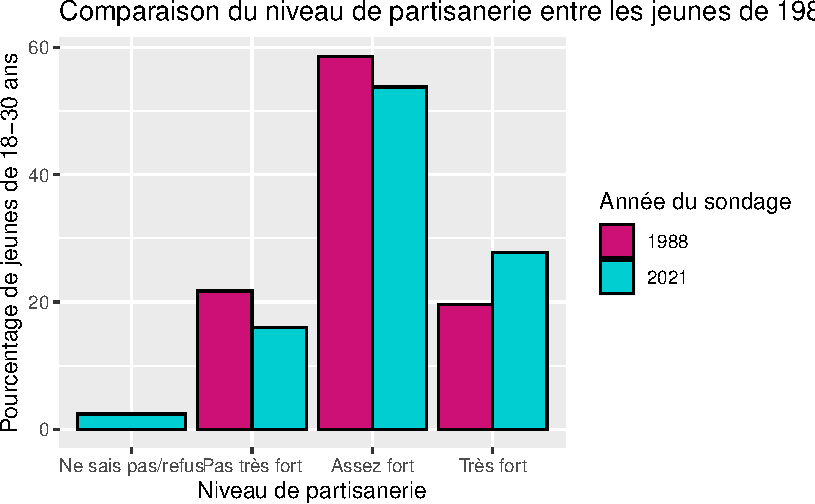
\includegraphics{TP2_FAS1001_Saffioti_files/figure-pdf/unnamed-chunk-1-1.pdf}

}

\end{figure}

\hypertarget{bibliograhie}{%
\subsection{Bibliograhie}\label{bibliograhie}}

Abramson, Paul R. 1976. «~Generational Change and the Decline of Party
Identification in America: 1952-1974~». \emph{The American Political
Science Review} 70 (2): 469‑78. \url{https://doi.org/10.2307/1959651}.

Converse, Philip E. 1976. ``The Dynamics of Party Support:
Cohort-Analyzing Party Identification''. Sage.

Lisi, M.2015. ``Partisanship and age effects in recent democracies:
Southern Europe from a comparative perspective''. \emph{Comparative
European Politics} 13(4) : 493-513.
\url{https://doi.org/10.1057/cep.2014.3}

Paugam, Serge. 2010. «~Méthodes~». In \emph{Les 100 mots de la
sociologie,} , 23‑43. Paris : Presses Universitaires de France.
\url{https://www.cairn.info/les-100-mots-de-la-sociologie--9782130574057-p-23.htm}.

Rettino-Parazelli, K. 2018. ``Les 18-35 ans : Portrait-robot d'une
génération courtisée par les partis politiques''. \emph{Le Devoir}, 17
août 2018.
\url{https://www.ledevoir.com/politique/quebec/534713/portrait-robot-d-une-generation}

Veilleux, Noémie. 2022. «~La partisanerie ne fait pas avancer le
Québec~». \emph{La Presse}, 31 août 2022.
\url{https://www.lapresse.ca/debats/opinions/2022-08-31/la-partisanerie-ne-fait-pas-avancer-le-quebec.php}.



\end{document}
